\documentclass[11pt, twocolumn]{article}
\usepackage[a4paper, hmargin={2.8cm, 2.8cm}, vmargin={2.5cm, 2.5cm}]{geometry}
%\usepackage[T1]{fontenc}
\usepackage[utf8]{inputenc}
\usepackage{eso-pic} % \AddToShipoutPicture
\usepackage{graphicx} % \includegraphics
\usepackage[english]{babel}
\usepackage{amssymb}
\usepackage{amsmath}
\usepackage{fancyhdr}
\usepackage{fancyvrb}
\usepackage{geometry}
\usepackage{listings}
\usepackage{cite}
\usepackage{subfigure}
\usepackage{color}
\usepackage{array}
\usepackage{multicol}
\usepackage[toc,page]{appendix}
\usepackage{cleveref}
\usepackage{hyperref}
\usepackage{float}
\usepackage{xcolor,colortbl}
\usepackage{pdfpages}
\usepackage{multirow}
\usepackage[font={small,it}]{caption}

\raggedbottom

%\nonstopmode

\newcommand\floor[1]{\lfloor#1\rfloor}

\definecolor{tablegreen}{rgb}{0.609375, 0.8828125, 0.3515625}
\definecolor{tableyellow}{rgb}{0.9921875, 0.859375, 0.2734375}
\definecolor{dkgreen}{rgb}{0,0.6,0}
\definecolor{gray}{rgb}{0.5,0.5,0.5}
\definecolor{mauve}{rgb}{0.58,0,0.82}


\newcolumntype{C}[1]{>{\centering\let\newline\\\arraybackslash\hspace{0pt}}m{#1}}
\setlength{\columnsep}{1cm}

\lstset{language=Python,
  aboveskip=3mm,
  belowskip=3mm,
  showstringspaces=false,
  columns=flexible,
  basicstyle={\small\ttfamily},
  numbers=none,
  numberstyle=\tiny\color{gray},
  keywordstyle=\color{blue},
  commentstyle=\color{dkgreen},
  stringstyle=\color{mauve},
  breaklines=true,
  breakatwhitespace=true,
  tabsize=4
}

\newcommand{\pic}[3] {
    \begin{figure}[ht]
        \centering
        \includegraphics[width=#3\textwidth]{#1}
        \caption{#2}
        \label{fig:#1}
    \end{figure}
}


\newcommand{\picappendix}[3] {
    \begin{figure}[H]
        \centering
        \includegraphics[width=#3\textwidth]{#1}
        \caption{#2}
        \label{fig:#1}
    \end{figure}
}

\newcommand{\asmcode}[3] {
    % \begin{figure}[H]
        % \centering
        \begin{Verbatim}[fontsize=\scriptsize]
        #3
        \end{Verbatim}
        \caption{#2}
        \label{fig:#1}
    % \end{figure}
}

\newcommand{\dpic}[5] {
    \begin{figure}[h]
\centering
\begin{subfigure}{#5\textwidth}
  \centering
  \includegraphics[width=.9\linewidth]{#1}
  \caption{#2}
  \label{fig:#1}
\end{subfigure}%
\begin{subfigure}{#5\textwidth}
  \centering
  \includegraphics[width=.9\linewidth]{#3}
  \caption{#4}
  \label{fig:#3}
\end{subfigure}
\end{figure}
}

\author{
\Large{
\begin{tabular}{C{4.5cm} C{4.5cm} C{4.5cm}}
  Jan Mezník \\
\texttt{PZJ895}
\end{tabular}
}
\vspace{12cm}
}

\title{
\vspace{3cm}
\Huge{Simulation of a MIPS machine} \\
\vspace{0.5cm}
%\Large{TEXT HERE}
}

\begin{document}


\onecolumn


%%%%% KU HEADER %%%%%%%%%%%%%%%%%%%%%%%
%% Change `ku-farve` to `nat-farve` to use SCIENCE's old colors or
%% `natbio-farve` to use SCIENCE's new colors and logo.
\AddToShipoutPicture*{\put(0,0){\includegraphics*[viewport=0 0 700
600]{include/ku-farve}}}
\AddToShipoutPicture*{\put(0,602){\includegraphics*[viewport=0 600 700
1600]{include/ku-farve}}}

%% Change `ku-en` to `nat-en` to use the `Faculty of Science` header
\AddToShipoutPicture*{\put(0,0){\includegraphics*{include/ku-en}}}


%\clearpage
\maketitle
\pagenumbering{roman}
\thispagestyle{empty}
\newpage
%%%%%%%%%%%%%%%%%%%%%%%%%%%%%%%%%%%%%%%

\begin{abstract}
\thispagestyle{empty}
TODO

\end{abstract}

\newpage

\twocolumn

%\thispagestyle{empty}
\tableofcontents

\onecolumn
\newpage
\twocolumn

\clearpage
\pagenumbering{arabic}
\setcounter{page}{1}

\markboth{Name}{Report}
\noindent
%\underline{\textbf{Category}}\\
%Hardware emulation\\\\
%\underline{\textbf{Keywords}}\\
%Copenhagen, university, computer, science, simulation, MIPS


\section{Introduction}
This report describes the development of a MIPS simulator, intended to support
the operating system KUDOS. The simulator will be written in C, and will
support the most important processor features and I/O devices, required to run
KUDOS, such as the translation lookaside
buffer (TLB), memory management unit (MMU), user and kernel CPU modes,
multiple cores (SMP), and I/O device emulation. \\


\subsection{Motivation}
KUDOS is a small operating system skeleton intended to be used by students
attending operating system project courses at university of Copenhagen.
It is used to explore operating system concepts by extending and improving on
existing system.
Initially, KUDOS targets the MIPS32 architecture, which leverages on the
advantages of a
reduced instruction set computing --- RISC.\\
To ease the development and debugging of KUDOS, it is desireable to run the
operating system
in a simulated machine. This enables the students and other developers to
better inspect the state of the machine, as well as making up
for the difference in the hardware of the host machine.

\subsection{A simulator}
A simulator is a program or a machine, that models some key characteristics
and functions of a given target.  The purpose of a
simulator is to be able to look inside the simulation and inspect the properties
and behaviours, that would otherwise only be seen in the real target.
A possible by-product of a simulator is that the simulation model will emulate
the target and its behaviour, practically immitating the target.\\
An emulator, on the other side, is intended to only mimick the behaviour of
a target on the outside, not correctly reflecting the internal state of the target.
Emulators are often used as a substitute for the real targets.
The difference between emulation and simulation is therefore, that unlike simulating a system,
an emulator only imitates the outward behaviour of its target, and it is hard
to predict how the target would act internally.\\
For example, mobile developers often use an emulator to test their
applications.
Instead of having thousands of real smartphones, they can simply emulate\footnote{
To be precise, they are emulating the hardware devices, but the applications they
are testing, are being simulated.}
the devices on their computers, saving both time and money.\\
A common use of a simulator is in the aircraft business, where flight-simulators
are being used for both pilot training, engineering, design, and many other
purposes. While it gives a very good insight on how a simulated airplane might
react in given situations, it does not actually move the users from one point
to another.\\
The purpose of our project is to write a program used at the Computer Systems
course at Copenhagen University, that can emulate KUDOS, while at the same
time, exposes the internal workings of the machine, for the students and
other participants to inspect and study.\\
Our target is therefore to simulate the academically important and relevant
parts, while others will be emulated.





\section{CPU Architecture}
At the heart of every computer lies the Central Processing Unit (CPU),
which is
an electronic circuit that carries out the basic arithmethic- and logic
calculation as well as process and redirect input and output to other devices
in the computer, using the shared busses.

Most modern CPUs are contained on a very small, yet packed intergrated circuit
chip, which can also house memory caches, multiple cores, and other processing
units.

The functionality of all processors is fundamentally the same. The processor
executes some primitive operation by fetching an instruction in the form of
binary signals, act upon the instruction and store the result in either
one of the its registers, or in the main memory.

A single instruction does very little, but a collection of instructions
make up
a program. In the very early computing days, computers were programmed in an
assembly language, which is simply human-readable instruction code. As the
computers grew more powerful, more complex and much faster, larger programs could be
executed. Because it is hard and time-consuming to write programs using
only the
assembly language, compilers are used to remove this complexity. A
compiler takes a high-level language, such as C, C++ or Java, and creates the
corresponding assembly language program for the specific architecture,
containing the instructions. This assembly language file is in turn assembled
or translated to binary, that the particular CPU can understand.

Besides hiding the complexity of the underlying architecture away from the
programmer, it can usually also compile programs to multiple architectures as
well as optimising the code to run faster.

\subsection{Instruction Set Architectures}
The instructions supported by a particular processor is determined by the
Instruction Set Architecture (ISA), which is the specification of how the CPU
works. An ISA determines the instructions
supported, the registers available, memory architecture, addressing modes as
well as handling of interrupts.

There exists many different types of ISAs, with both their advantages and
disadvantages. For example, some architectures have a very few instructions
and registers, which is very practical for small embedded devices,
whereas large
servers might make use of a large array of registers for complex computations.

Besides the current use of an architecture, designers must also take into
account its future uses and applications. As the world of computation is ever
growing and evolving at exponential rates, the architectures must be up to the
challenge of future computing. Introducing a completely new architecture to
the market is very troublesome, and causes a list of problems.
One of the main issues is that old software written for older architectures
will no longer work, and it requires to be either recompiled, rewritten,
or even emulated. One such example is the Intel Itanium (IA-64) architecture,
which had a very bad marked reception due to its lack of backwards
compatibility
with the x86 architecture. The emulation of the architecture on IA-64 yielded
suboptimal performance and ultimately lost to the AMD x86\_64, which in
turn was
compatible.\cite{anandtech:1854}

Indeed, there are a lot of factors to take into account when designing a new
architecture, and every decision has big implications on the future of the
whole ISA.

\subsection{MIPS Architecture}
The MIPS architecture (acronym for Microprocessor without Interlocked Pipeline
Stages) was first created in the early 1980s.\cite{imgtec:MIPS_Overview}
MIPS is a reduced instruction set architecture (RISC), developed by MIPS
technologies, to bring new levels of
performance and efficiency into the world of processing units. As an RISC
architecture, MIPS aims to implement only the most essential instructions, so
that they in return can get highly optimised. This is the based on the RISC
philosophy, that by implementing only the most common instructions, the
architects can simplify the design and speed up the crucial parts of the
instructions. This enables the processor to execute programs faster, but also
removes a lot of complexity of implementing large programs.

In contrast to RISC, complex instruction set architecture (CISC) aims
to reduce the number of instructions needed to execute a program by
implementing instructions packed with functionality. This means that a single
instruction in CISC can execute several operations at once, such as loading
from memory, arithmetic
and storing. While complex programs indeed execute faster on a CISC
architecture,
the burden of implementing efficient and maintainable code and compilers can
outweigh its advantages. \cite{Patterson:1980:CRI:641914.641917}

Besides the inspiration from RISC, MIPS has added its own design principles,
which are honored and used to question every change, implementation,
or design.
These are \cite{COD5}:
\begin{itemize}
	\item \textit{Design Principle 1:} Simplicity favors regularity.
	\item \textit{Design Principle 2:} Smaller is faster.
	\item \textit{Design Principle 3:} Good design demands good
	compromises.
	\item \textit{Design Principle 4:} Make common case fast.
\end{itemize}
These decisions withstood the trial by fire and proved, that honoring these
principles yields good design, easing implementation as well as simplifying
hardware.


\section{MIPS Core Processing Unit}
MIPS CPUs are pipelined, meaning that it implements a pipeline which
enables it
to execute different stages of multiple instructions at once. This gives the
processor a higher throughput that would otherwise be possible at a given
clock-rate. The processor has 31 general purpose (GP) registers, with
additional registers
per co-processing unit. Even the first models of the MIPS CPUs, such as the
MIPS R2000, had memory caches and a translation lookaside-buffer, which improves
the speed of the processor by reducing the number of main memory lookups.

\subsection{Registers}
MIPS contains multiple types of registers. The most common and most used
registers are the general-purpose registers (GP), which can be used for
practically anything by the programmer. Special registers are registers
implemented for cases where GP registers were either too small or otherwise
unsuitable for the purpose.\\
For additional functionality, the MIPS co-processor 0 also has its own set of
registers that, along with an operating system, bring many features to the
system.

\subsubsection{General Purpose Registers}
In MIPS, there are 32 general-purpose registers, all 32 bit wide. Although
they
can all theoretically be used however the programmer or assembler
wants\footnote{Except the 0'th (\$0) register, which can only hold the
value 0.}, there
are some conventions for the use of the registers.
\begin{center}
    \begin{tabular}{ | l | l | l | c |}
    \hline
	\textbf{Mnemonic\footnote{Textual mnemonic used in the assembly language}}%
		 & \textbf{\#} & \textbf{Use} \\ \hline \hline
	\texttt{\$zero}		& 0	& Constant Value 0 \\ \hline
	\texttt{\$at}		& 1	& Reserved Temporary \\ \hline
	\texttt{\$v0-\$v1}	& 2-3	& Function Results \\ \hline
	\texttt{\$a0-\$a3}	& 4-7	& Function Arguments \\ \hline
	\texttt{\$t0-\$t7}	& 8-15	& Temporaries  \\ \hline
	\texttt{\$s0-\$s7}	& 16-23 & Saved Temporaries \\ \hline
	\texttt{\$t8-\$t9}	& 24-25 & Temporaries \\ \hline
	\texttt{\$k0-\$k1}	& 26-27 & Reserved for OS \\ \hline
	\texttt{\$gp}		& 28	& Global Pointer \\ \hline
	\texttt{\$sp}		& 29	& Stack Pointer \\ \hline
	\texttt{\$fp}		& 30	& Frame Pointer \\ \hline
	\texttt{\$ra}		& 31	& Return Address \\ \hline
    \end{tabular}
\end{center}

\subsubsection{Special Registers}
The special registers in MIPS cannot directly be accessed from the program.
Rather, they are modified by different instructions.
\begin{center}
    \begin{tabular}{ | l | l | l | c |}
    \hline
	\textbf{Name} & \textbf{\#} & \textbf{Use} \\ \hline \hline
	\texttt{HI}		& -	& Hi-word of 64bit value \\ \hline
	\texttt{LO}		& -	& Lo-word of 64bit value \\ \hline
	\texttt{\$PC}		& -	& Program Counter \\ \hline
    \end{tabular}
\end{center}
\texttt{HI} and \texttt{LO} registers are used to contain the result of a
multiplication or division, which, using 2 32bit registers, can end with a
64bit result.\\
The PC register is pretty self-explanatory, as it simply points the current
location in the program (or "counts" the instructions). On other
architectures,
this register is better known as the Instruction Pointer (IP).

\subsubsection{Co-processor 0 registers}
Registers in co-processor 0 are mainly used by the system, to provide
additional features. The co-processor can have 32 registers, but only few of
them are used consistently. Many of the empty registers are also defined
by the
manufacturer of the processor.
\begin{center}
    \begin{tabular}{ | l | l | l | c |}
    \hline
	\textbf{Name} & \textbf{\#} & \textbf{Use} \\ \hline \hline
	\texttt{index}		& -	& TLB entry index\\ \hline
	\texttt{random}		& -	& TLB random access register \\ \hline
	\texttt{entrylo}	& -	& Low order current TLB entry \\
	\hline
	\texttt{context}	& -	& Page-Table lookup addr. \\ \hline
	\texttt{vaddr}		& -	& Virtual address of exceptions
	\\ \hline
	\texttt{entryhi}	& -	& High order current TLB entry\\
	\hline
	\texttt{status}		& -	& Processor status \\ \hline
	\texttt{cause}		& -	& Exception cause \\ \hline
	\texttt{epc}		& -	& PC when exception occured \\ \hline
    \end{tabular}
\end{center}
The \texttt{status} register is a bit-field of flags used to signal the
current
state of the processor. It is similar to the \texttt{EFLAGS} register on
x86 architectures.

The rest of the registers will be discussed in depth in the SMP chapter.


\subsection{Instructions}
Each instruction in MIPS is 32-bit long, aligned to word. This simplifies the
instruction fetching, decoding, as well as disassembly of the program,
for both
the processor as well as the programmer.

In MIPS, the instructions have 3 basic formats:
\begin{figure}[H]
\centering
\subfigure[R-Format]{%
	
\includegraphics{cpu_architecture/r_format.eps}
	\label{fig:instruction_r_format}}
\subfigure[I-Format]{%
	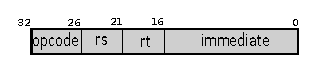
\includegraphics{cpu_architecture/i_format.eps}
	\label{fig:instruction_i_format}}
\subfigure[J-Format]{%
	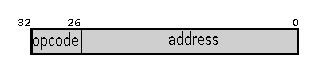
\includegraphics{cpu_architecture/j_format.eps}
	\label{fig:instruction_j_format}}
\label{fig:instruction_formats}
\end{figure}

It is clear that, as they have common fields, mainly the opcode field,
they are
easily distinguishable.\\
The R-format instructions are mainly used when all the data being processed is
located in the registers. That includes adding between registers, binary
operations on values in registers as well as jumping to an address located in
a register.\\\\
The I-format instructions can operate on both data from registers and
immediate
values encoded directly in the instruction (thus the 16-bit immediate field).
I-format instruction share a lot of common operations with the R-format, where
one of the operands is the immediate.\\\\
J-format instructions are used solely for jumping instructions, thus the large
address field. As it only has 26 bits to address an 32 byte memory location, it
shifts the whole value twice to the left, as to align the value in words. The
upper 4 bits are retrieved from PC. In practise, this is enough to jump to any
address in the program.

\subsection{Arithmetic Logic Unit}
Without any extension co-processing unit, the Arithmentic Logic Unit (ALU) in
MIPS32 only supports operations on integers. \\
The ALU supports basic mathematical operations such as adding (\texttt{add}),
subtracting (\texttt{sub}), as well as logical shifting to both left and right
(\texttt{sll, srl}), which also can be used to division or multiplication by
even numbers.

All bitwise logical operators \texttt{and, or, and nor} are implemented Using
these, which additional missing logical operations can be created, such as
\texttt{nand} and \texttt{not}.\\
Since both the operand and destination registers are 32 bit wide, an overflow
in the result might occur - that is, the result is larger than what a 32 bit
register can hold.
In that situation, an exception is raised in the processor, and code to recover
from this error is run\cite{COD5}. This will be explained in later sections.


\subsection{Load and Store}
MIPS is a "load/store" architecture, where memory is only accessed by specific
load and store instructions \cite{flynn1995computer}. This design is a very
common for RISC architectures, as it greatly simplifies the pipeline stages and
clock timings. In contrast, CISC architectures have many instructions that can
do operations on both memory and registers at the same time. For example, on
the x86\_64 architecture, the
\texttt{MOVSW} instruction reads from a memory location pointed to by register
SI, stores it in memory location DI, and at last, increments (or
decrements\footnote{This is determined by the direction flag, which determines
whether the CPU reads memory from top to bottom or in reverse.})
both registers\cite{intelmanual}. This adds additional stall and hazard logic to
the processor, and makes it is hard for the CPU to determine how many
clock-ticks the instruction will take.\\\\
MIPS32 uses \texttt{lw} for loading a word from the main memory into the register,
and a \texttt{sw}, which stores the value from register into the specified
memory location. In reality, MIPS32 also has \texttt{LH}, \texttt{LB} and
their store counterparts \texttt{SH} \texttt{SB}, which operate on half-word
and byte sized loads and stores. However, for performance reasons, the main
memory always reads a word (4 bytes), and so, the desired size is computed in
the CPU.



\subsection{Jumping and Branching}
To be turing complete, the processor needs to be able to do conditional jumps
to other memory locations. This is done with the jumping instructions: jump
(\texttt{j}), jump-register (\texttt{jr}) and jump-and-link (\texttt{jal}). The
conditional jumps are: branch-equal (\texttt{beq}) and branch-not-equal
(\texttt{bne}).\\
On the bare-metal level of the processor, these instructions simply modify the
value of the Program Counter register, which is otherwise inaccessible from
assembly.

\subsection{Interrupts}
Interrupts is a special way to control what the CPU. It actively "interrupts"
the CPU from its current job, and makes it execute a special function,
specified by an interrupt number. There usually 3 types of interrupts\cite{osdev:interrupts}:
\begin{itemize}
	\item Exceptions\\
	Exceptions occur in software, usually when an error has occurred that
	needs attention from the kernel. This is usually caused by reading from
	illegal memory addresses or when arithmetic overflow occurs.

	\item Hardware Interrupt\\
Hardware interrupts are initiated from hardware devices, such as a
mouse or a keyboard. When a user presses a key or moves the mouse, the hardware
devices send a signal to the CPU that something has happened that needs
attention from the kernel.

	\item System Call (syscall)\\
	Syscalls are usually used by programs, when they need attention from
the kernel. An operating system and the underlying kernel will usually expose
an interface with a whole set of functions, that the program can access by
syscalls. This can be everything from reporting termination of a program to
writing data to the disk.
\end{itemize}

The action that the CPU has to perform is determined by an interrupt vector
table. For each interrupt vector, there is specific code to be executed.
Because the interrupt vector table is limited in size, operating systems, such
as Linux, use a single interrupt vector number 0x80. Additional arguments for
further determination of the service are passed in service number, which is
stored in the general purpose registers, and if needed, in the stack.\\
System call handling is made somewhat easier in MIPS. Whereas in x86\_64, you
have to set the appropriate system-calls arguments and then do an interrupt on
the correct vector, MIPS has a dedicated system-call instruction
\texttt{syscall}. The operating system can choose however the arguments are
passed, but usually, the service number is stored in \texttt{\$v0}, and the
arguments in \texttt{\$a0-\$a3}\cite{COD5}.



% MIPS supports up
%to 4 coprocessors (COP), with each COP extending on the basic functionality. The
%only required co-processor is COP0, which is the System Control Coprocessor.
%Other co-processors usually available, but not required, are the floating-point operation
%coprocessor COP1 (FPU), the user defined COP2.





\section{TLB}

\section{MMU}

\section{User and Kernel mode}

\section{SMP}

\section{Tests}

\section{Performance}

\section{Conclusion}


\newpage

\bibliography{mybib}{}
\bibliographystyle{plain}

\newpage

\appendix
\begin{appendices}
% Appendix here
\end{appendices}

\end{document}
